% EN49 c07 | 原书 p.65–75（PDF 76–86） | 第 4 章 §4.2
% 骨架文件：标题行已设定，正文由译者填写。每页起首用 % ===== 原书 p.N ===== 注释标记。
\subsection{主定理的证明}

% ===== 原书 p.65 =====
后文我们将在关于 $f$、$g$ 与 $X$ 的强假设下证明：相对 Fukaya--Seidel 范畴确实等价于
Fukaya--Seidel 范畴 $\cW(X,f+\delta g)$，其中 $\delta>0$ 充分小。一般而言这个等价当然
不应成立。

由于这一构造，定理 \ref{thm:aak-equiv} 的证明可以原样搬来，说明在临界轨迹中的可容
拉格朗日子流形上取顶针，给出全忠实函子
\[
T\colon\cW(f^{-1}(t),g)\to\cW(X\times\C,z(f-t),g).
\]
在适当修改命题 \ref{prop:3-0-5} 之后，我们预期它是一个等价。

由于要考虑两个 Landau--Ginzburg 模型，为相应的 cap 函子与 cup 函子建立记号很重要：

\begin{itemize}
\item 对 Landau--Ginzburg 模型 $(X,f)$，我们用
$\cap\colon D\cW(X,f)\to D\cW(f^{-1}(t))$，\\
与 $\cup\colon D\cW(f^{-1}(t))\to D\cW(X,f)$；
\item 对 Landau--Ginzburg 模型 $(X\times\C,F_t)$，则改用记号
$\bigcap\colon D\cW(X\times\C,F_t)\to D\cW(X\setminus f^{-1}(t))$，\\
与 $\bigcup\colon D\cW(X\setminus f^{-1}(t))\to D\cW(X\times\C,F_t)$。
\end{itemize}

\transnote{易错预警：本节的 cap 与 cup 函子有两套记号。模型 $(X,f)$ 用小的
$\cap$、$\cup$；模型 $(X\times\C,F_t)$ 用大的 $\bigcap$、$\bigcup$。文字层把大符号识别成
拉丁字母 T 与 S，对照页图时务必分清：正文里的 $\bigcup\ell$ 不是「$S\ell$」，
$\bigcap$ 也不是 AAK 等价里的函子 $T$。}

我们将经命题 \ref{prop:3-0-5} 构造的 Viterbo 限制映射（Viterbo restriction map），把
$D\cW(X\setminus f^{-1}(t),f)$ 的对象看作 $D\cW(X,f)$ 的对象。

我们的结果将由下述事实推出：在定理 \ref{thm:aak-equiv} 的 AAK 等价下，作用于附加手柄
的余核 $\ell\subseteq X$ 的 cap 函子

% ===== 原书 p.66 =====
$\cap\colon\cW(X,f)\to\cW(f^{-1}(t))$ 所给出的对象，在 $\cW(X\times\C,z(f-t))$ 中同构于
该附加手柄的核心关于 $X\setminus f^{-1}(t)$ 上 Liouville 结构的环绕圆盘。由
[GPS19, §7.2]，这些手柄的环绕圆盘由 cup 函子
$\bigcup\colon\cW(X\setminus f^{-1}(t))\to\cW(X\times\C,z(f-t))$ 作用于手柄的余核 $\ell$
给出。因此该同构正是 [AS15, Lemma A.28]；可惜其中勾勒的证明难以严格化。该同构也可由
[AG] 中构造的伴随给出的大形式论证推出。这里我们给出一个不依赖 [AG] 的替代论证。

\transnote{背景直觉：这一步要把「环绕圆盘」与「余核在 cap 函子下的像」等同起来，本质上是
把手柄分解一侧的几何翻译成 Fukaya 范畴里的对象。Yoneda 引理随后把对象层面的同构升级为
左模的同构，这才足以锁定 $A_\infty$ 结构。}

对 $A_\infty$ 范畴使用 Yoneda 引理 [Sei08b, Corollary 14.7]，我们要证的便是：

\begin{theorem}\label{thm:4-2-1}
对每个附加余核 $\ell$，存在 $\cW(f^{-1}(t))$ 上左模（left module）的等价
\[
T^*\cY_{\bigcup(\ell)}\cong\cY_{\cap\ell},
\]
其中 $\cY\colon\cW(f^{-1}(t))\to\cW(f^{-1}(t))\mathrm{Mod}$ 是左 Yoneda 函子（left Yoneda functor），
$T^*$ 表示左模的拉回。
\end{theorem}

\transnote{含糊点拨：记号 $\cW(f^{-1}(t))\mathrm{Mod}$ 指该范畴上左模范畴，$\mathrm{Mod}$
用直立体、不加空格。$T^*$ 只在左模层面有定义（不是几何上的拉回），故本定理的比较发生在
模范畴里。}

\begin{proof}
本证明继续使用上面在 $X\times\C$ 上构造的 Liouville 结构。注意关于诱导的 Liouville
结构，$F_t$ 的每个纤维都含一个微分同胚于 $f^{-1}(t)\times\C^*$ 的开邻域，其中的
Liouville 向量场由与标准 Liouville 向量场的乘积给出：
\[
Z=-\frac{\varepsilon}{r^3}\partial_r,
\]
其中 $r=|z|$ 是径向坐标。

% ===== 原书 p.67 =====
给定 $\cW(f^{-1}(t))$ 中任一拉格朗日子流形 $L$，顶针 $TL$ 与 $\bigcup\ell$ 在 $F_t$ 的
同一个纤维中相交，设在 $0<\delta\in\C$ 所对应的纤维上；这里取 $\delta>0$ 充分小，使
$B_\delta$ 上方 $TL$ 完全落在 Morse--Bott 模型内。由于乘积结构，在纤维
$F_t^{-1}(\delta)$ 中 $TL$ 由 $L\times K\subseteq f^{-1}(t)\times\C^*\subseteq
X\setminus f^{-1}(t)$ 给出，其中 $K\subseteq\C^*$ 是绕 $0$ 的小圆周。按 cup 函子的
定义，$\bigcup\ell$ 在该纤维 $F_t^{-1}(\delta)$ 中正好由余核 $\ell$ 给出；见
图 \ref{fig:mod-gvs}。

\transnote{易错预警：原文写「$0<\delta\in\C$」，$\C$ 上并没有序，这里的 $\delta$ 实际是
小的正实数，只是借用 $\C$ 的实轴来定位纤维。译文照录，读者按正实数理解即可。}

注意到在命题 \ref{prop:3-0-3} 对 $X\setminus f^{-1}(t)$ 上 Stein 结构的分析中，每个
附加余核的边界必落在 $f^{-1}(t)$ 中：它们不能留在紧集内，因为 Stein 函数没有指标
$(n+1)$ 的临界点；它们也不能以 $|f-t|^{-1}(\delta)$ 为边界，因为 Liouville 向量场指向
内部。我们在 $X\times\C$ 上用来定义 Fukaya 范畴的 Liouville 结构是该 Stein 结构的形变，
但这个正合形变保持 Liouville 向量场的流线。由于 Liouville 向量场在
$f^{-1}(t)\times\C^*\subseteq X\setminus f^{-1}(t)$ 上的局部形状，这意味着 $\ell$
纤维化于 $\C^*$ 之上，因而与 $L\times K$ 在 $f$ 的同一个纤维中相交。在该纤维内，按 cap
函子的定义，$\bigcup\ell$ 由 $\cap\ell$ 给出；因此 $TL$ 与 $\bigcup\ell$ 正好沿
$L\cap(\cap\ell)\subseteq f^{-1}(t)$ 相交；见图 \ref{fig:mod-gvs}。于是得到向量空间的
同构：
\[
T^*\cY_{\bigcup(\ell)}(L)=CF\left(\bigcup\ell,TL\right)
\cong CF(\cap\ell,L)=\cY_{\cap\ell}(L).
\]
又由马斯洛夫指数在乘积下的可加性，这实际上是分次向量空间的同构。还需匹配
$A_\infty$ 模运算 $\mu^k$。

\transnote{含糊点拨：$|f-t|^{-1}(\delta)$ 指函数 $|f-t|$ 的 $\delta$ 水平集，与纤维
记号 $f^{-1}$ 不是一回事；原文两种上标 $-1$ 混用，中文只能照译并在此提示。}

我们从微分 $\mu^1$ 开始。此时 $TL$ 与 $\bigcup\ell$ 的交集落在纤维 $f^{-1}(t)$ 内，而该
纤维含于 $F_t^{-1}(\delta)$ 中。

% ===== 原书 p.68 =====
\begin{figure}[htbp]
\centering
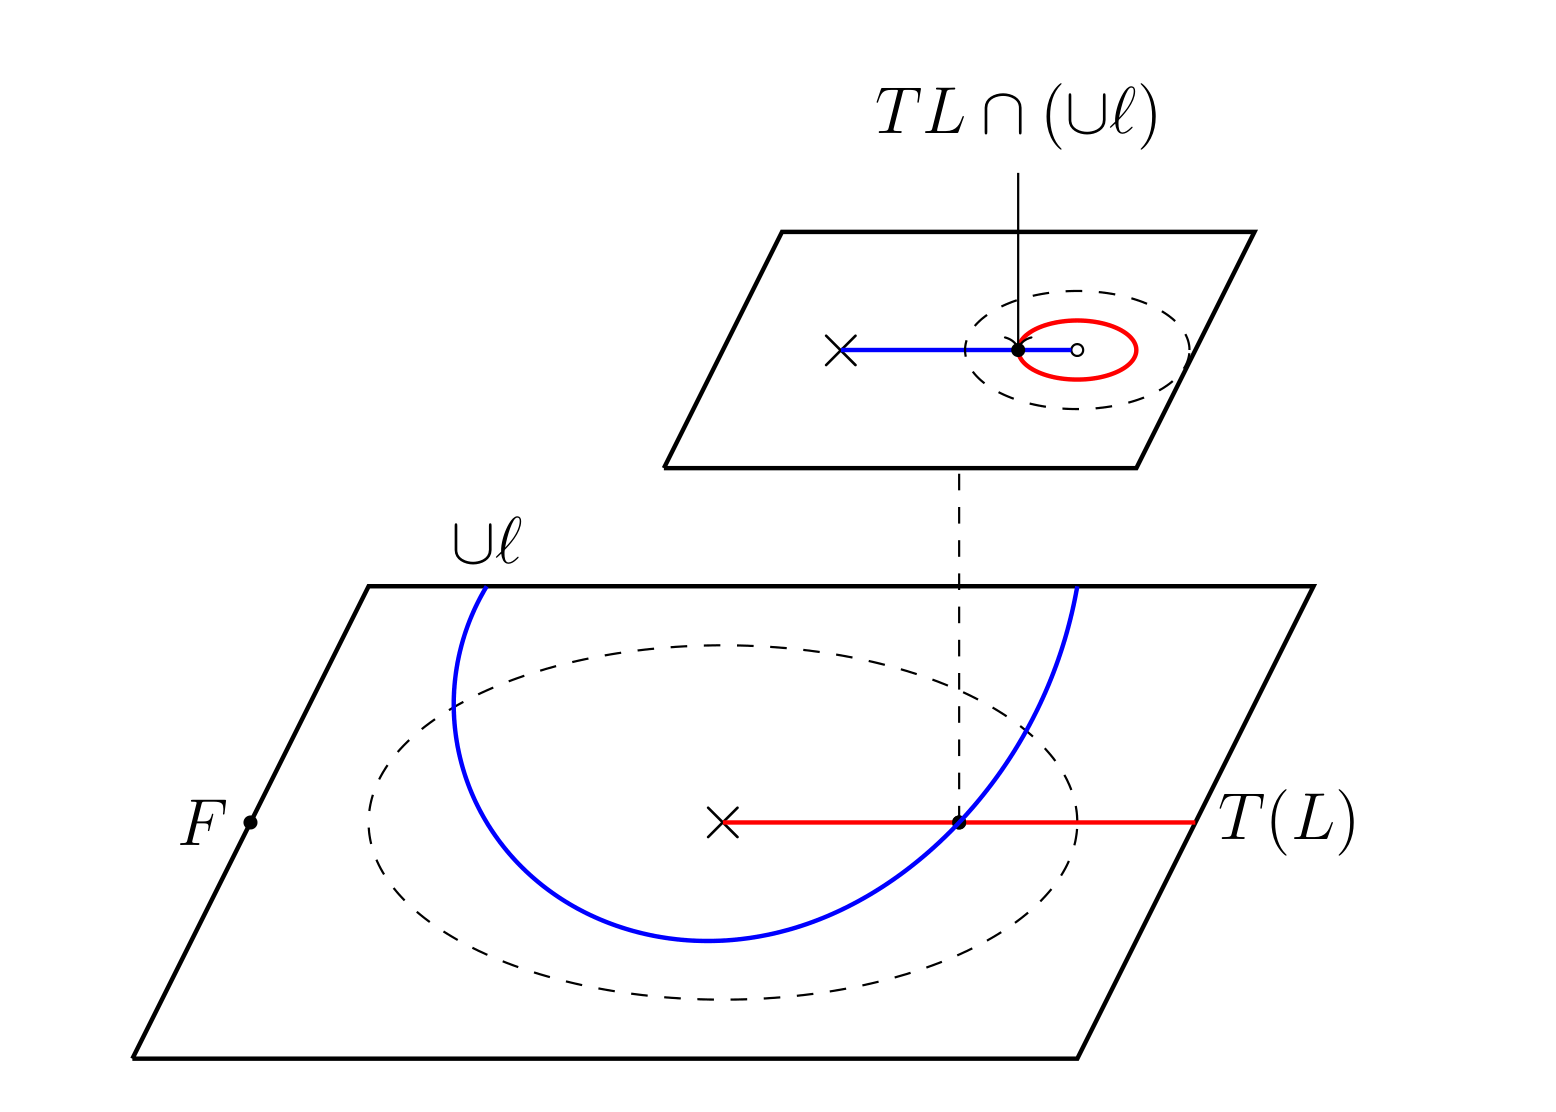
\includegraphics[width=0.72\textwidth]{figures/fig4_2.png}
\caption{把各模识别为分次向量空间。}
\label{fig:mod-gvs}
\end{figure}

把定理 \ref{thm:aak-equiv} 中的极大值原理论证迭代用于全纯映射 $F_t$ 与 $f$，即知计算
$\mu^1\colon T^*\cY_{\bigcup(\ell)}(L)\to T^*\cY_{\bigcup(\ell)}(L)$ 的全纯圆盘全部落在
该纤维 $f^{-1}(t)\subseteq F_t^{-1}(\delta)$ 内；再把那里的横截性论证稍作变化便知，任何
用于使 $f^{-1}(t)$ 内圆盘横截的近复结构，都可延拓到 $X\times\C$，使总空间中计算 $\mu^1$
的圆盘也正则。

\transnote{易错预警：这里用的是定理 \ref{thm:aak-equiv} 证明中「极大值原理把圆盘压进
$F_t^{-1}(0)$、再压进 $f^{-1}(t)$」的迭代版本；两次极大值原理对应两次投影（$F_t$ 与
$f$），不要误当作一次。}

现在把乘积运算 $\mu^2$ 当作后续论证的简化原型。设 $L_1,L_2$ 是 $f^{-1}(t)$ 中的正合
柱状拉格朗日子流形，令 $T^{(i)}L_i=T_i^{(i)}$ 为它们如定理 \ref{thm:aak-equiv} 的证明中
那样的顶针。设有交点 $y_1\in(\cap\ell)\cap L_1$、$x\in L_1\cap L_2$ 与
$y_2\in T^{(2)}L_2\cap(\cap\ell)$，并对定义以下运算的圆盘模空间
$\cM_J^{f^{-1}(t)}(y_1,x,y_2)$，在 $f^{-1}(t)$ 上选取正则的近复结构 $J$（依赖于定义域
与共形结构）：

% ===== 原书 p.69 =====
\[
CF(L_2,L_1)\otimes\cY_{\cap\ell}(L_2)\to\cY_{\cap\ell}(L_1).
\]

把这些近复结构延拓为 $X\times\C$ 上的近复结构，使其在邻域 $f^{-1}(t)\times\C$ 上为
乘积型；延拓后的结构仍记为 $J$。

由定理 \ref{thm:aak-equiv} 与上述论证，这些交点对应于以下交点：
$y_1\in\bigcup\ell\cap T^{(1)}L_1$，落在 $F_t^{-1}(\delta)$ 中；
$x\in T^{(1)}L_1\cap T^{(2)}L_2$，落在 $F_t^{-1}(0)$ 中；以及
$y_2\in T^{(2)}L_2\cap\bigcup\ell$，按顶针 $T_i^{(i)}$ 的构造落在
$F_t^{-1}(e^{i\theta}\delta)$ 中，其中 $0<\theta<\pi$。现在考虑 $X\times\C$ 内与下述
运算相对应的全纯圆盘模空间 $\cM_J^{X\times\C}(y_1,x,y_2)$：
\[
CF(T^{(2)}L_2,T^{(1)}L_1)\otimes\cY_{\bigcup\ell}(T^{(2)}L_2)
\to\cY_{\bigcup\ell}(T^{(1)}L_1).
\]

所有这些交点都落在局部 Morse--Bott 模型 $f^{-1}(t)\times\C^2$ 内。于是对全纯映射
$F_t$ 与 $f$ 的投影施用 $\C$ 上标准近复结构的极大值原理，所有这些圆盘必落在局部
Morse--Bott 邻域 $f^{-1}(t)\times\C^2\subseteq F_t^{-1}(B_\delta)$ 内。在这个
Morse--Bott 模型内，我们有若干全纯投影。首先，投影到 $f^{-1}(t)$ 给出满射
\[
p\colon\cM_J^{X\times\C}(y_1,x,y_2)\to\cM_J^{f^{-1}(t)}(y_1,x,y_2),
\]
这是因为近复结构就是这样定义的。我们断言它实际上是双射，并且
$\cM_J^{X\times\C}(y_1,x,y_2)$ 关于该近复结构正则。

% ===== 原书 p.70 =====
为看出这一点，设 $(u,r)\in\cM_J^{X\times\C}(y_1,x,y_2)$ 是这样的圆盘，
$u\colon D\to X\times\C$，而 $r$ 是三标点圆盘 $D$ 的唯一共形类（conformal class）；那么可以证明，它由到
$f^{-1}(t)$ 的投影决定，如下。

令 $\pi\colon f^{-1}(t)\times\C^2\to\C^2$ 为到第二个因子的（全纯）投影。考虑从三标点
圆盘 $D$ 到 $\C^2$ 的全纯映射 $\pi\circ u$。由于三标点圆盘的共形等价类唯一，这个全纯
圆盘 $(\pi\circ u,r)$ 计算运算
\[
\mu^2\colon CF(T_2,T_1)\times CF(U,T_2)\to CF(U,T_1),
\]
其中 $T_i,U\subseteq\C^2$ 分别是投影 $\pi(T^{(i)}L_i)$、$\pi(\bigcup\ell)$ 所得的
拉格朗日子流形；见图 \ref{fig:mu2}。这些 $T_i$ 是 $\C^2$ 上标准 Lefschetz 纤维丛的
顶针，因而在原点横截相交。拉格朗日子流形 $U$ 是实轴 $\R_+$ 在模型 Lefschetz 纤维丛
一般纤维 $\{z_1z_2=\delta\}\cong\C^*$ 内的平行移动，因而与每个 $T_i$ 各横截相交于一点。

\transnote{背景直觉：在 $\C^2$ 的模型里，$T_i$ 是 Lefschetz 顶针、$U$ 是实轴的平行
移动，后者与每个顶针恰好横截交于一点。正因为交点如此之少，$\C^2$ 里的模空间只有单个
正则圆盘，$\pi$ 才可能是双射。}

对 $\C^2$ 上一般的近复结构 $J$，该模空间由单个正则圆盘组成，它计算唯一交点
$p\in U\cap T_1$ 与 $T_1\cong T_2$ 的恒等元的乘积。把前面关于 $X\times\C$ 上近复结构的
构造用于此处的 $J$（代替 $\C^2$ 上标准近复结构），便知可以保证：对任何
$(u,r)\in\cM_J^{X\times\C}(y_1,x,y_2)$，$p(u,r)$ 与 $\pi(u,r)$ 都正则。这恰好说明，在
$p$ 下任何 $\cM_J^{f^{-1}(t)}(y_1,x,y_2)$ 中圆盘的原像里只有一个全纯圆盘。容易验证这些
模空间上诱导的定向一致。

对更高的 $\mu^k$ 运算，我们先推广上述关于 $\mu^2$ 的论证。设 $L_i$（$i=1,\dots,k$）
是 $f^{-1}(t)$ 中的正合柱状拉格朗日子流形，并令 $T^{(i)}L_i=T_i^{(i)}$ 为它们如
定理 \ref{thm:aak-equiv} 证明中那样的顶针。

% ===== 原书 p.71 =====
\begin{figure}[htbp]
\centering
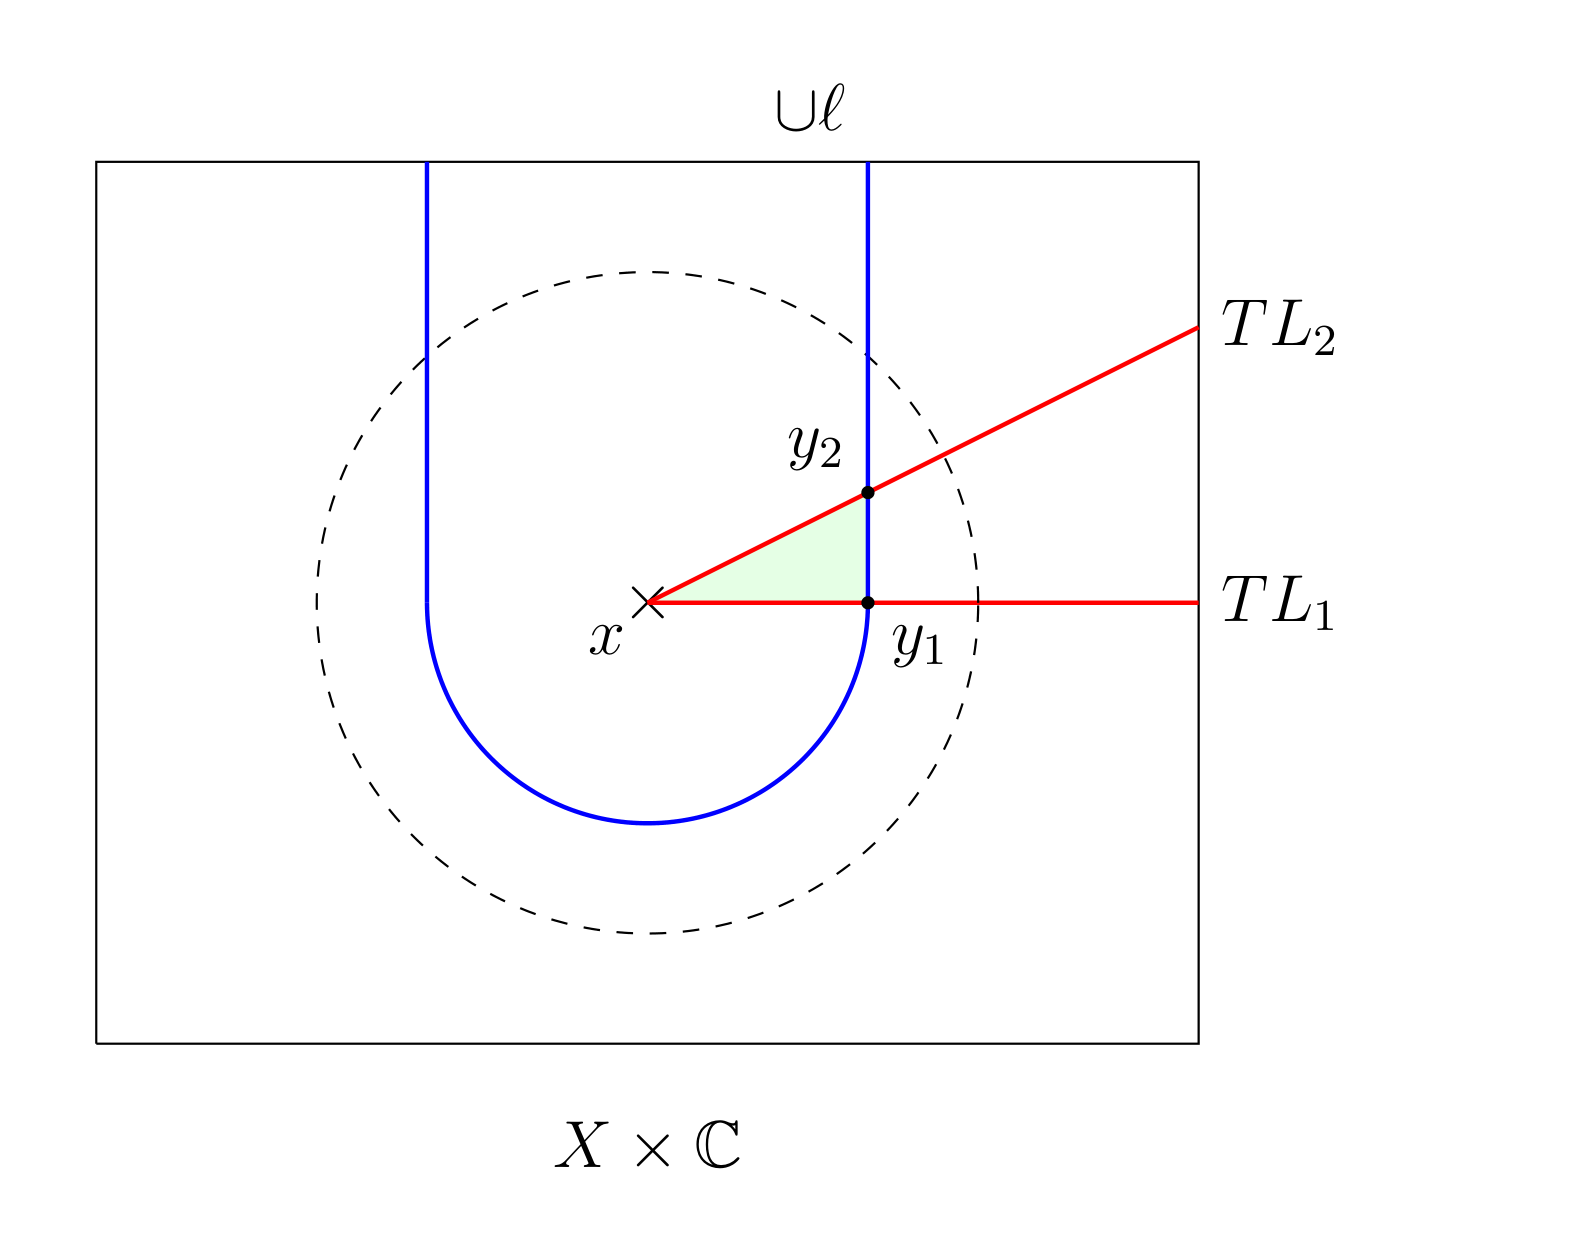
\includegraphics[width=0.72\textwidth]{figures/fig4_3.png}
\caption{把模上的 $\mu^2$ 运算识别出来：绿色部分是那个全纯圆盘。}
\label{fig:mu2}
\end{figure}

设有交点 $y_1\in(\cap\ell)\cap L_1$、$x_i\in L_i\cap L_{i+1}$（$i=1,\dots,k-1$）与
$y_2\in T^{(k)}L_k\cap(\cap\ell)$，并对定义以下运算的圆盘模空间
$\cM_J^{k,f^{-1}(t)}(y_1,x_1,\dots,x_k,y_2)$，在 $f^{-1}(t)$ 上选取正则的近复结构
$J$（依赖于定义域与共形结构）：
\[
CF(L_2,L_1)\otimes\cdots\otimes CF(L_k,L_{k-1})\otimes\cY_{\cap\ell}(L_k)
\to\cY_{\cap\ell}(L_1).
\]
把这些近复结构延拓为 $X\times\C$ 上的近复结构，使其在邻域 $f^{-1}(t)\times\C$ 上为
乘积型。

% ===== 原书 p.72 =====
由定理 \ref{thm:aak-equiv} 与上述论证，这些交点对应于以下交点：
$y_1\in\bigcup\ell\cap T^{(1)}L_1$，落在 $F_t^{-1}(\delta)$ 中；
$x_i\in T^{(i)}L_i\cap T^{(i+1)}L_{i+1}$（$i=1,\dots,k-1$），落在 $F_t^{-1}(0)$ 中；
以及 $y_2\in T^{(k)}L_k\cap\bigcup\ell$，按顶针 $T_i^{(i)}$ 的构造落在
$F_t^{-1}(e^{i\theta}\delta)$ 中，其中 $0<\theta<\pi$。现在考虑 $X\times\C$ 内与下述
运算相对应的全纯圆盘模空间
$\cM_J^{k,X\times\C}(y_1,x_1,\dots,x_k,y_2)$：
\[
\begin{gathered}
CF(T^{(2)}L_2,T^{(1)}L_1)\otimes\cdots\otimes
CF(T^{(k)}L_k,T^{(k-1)}L_{k-1})\\
\otimes\cY_{\bigcup\ell}(T^{(k)}L_k)\to\cY_{\bigcup\ell}(T^{(1)}L_1).
\end{gathered}
\]

所有这些交点都落在局部 Morse--Bott 模型 $f^{-1}(t)\times\C^2$ 内。于是对全纯映射
$F_t$ 与 $f$ 的投影施用 $\C$ 上标准近复结构的极大值原理，所有这些圆盘必落在局部
Morse--Bott 邻域 $f^{-1}(t)\times\C^2\subseteq F_t^{-1}(B_\delta)$ 内。在这个
Morse--Bott 模型内，我们有若干全纯投影。首先，投影到 $f^{-1}(t)$ 给出满射
\[
p\colon\cM_J^{k,X\times\C}(y_1,x_1,\dots,x_k,y_2)\to
\cM_J^{k,f^{-1}(t)}(y_1,x_1,\dots,x_k,y_2),
\]
这是因为近复结构就是这样定义的。我们断言它实际上是双射，且
$\cM_J^{k,X\times\C}(y_1,x_1,\dots,x_k,y_2)$ 关于该近复结构正则（如前，可以验证这些
模空间上诱导的定向一致）。为说明这一点，设
$(u,r)\in\cM_J^{k,X\times\C}(y_1,x_1,\dots,x_k,y_2)$ 是这样的圆盘，
$u\colon D\to X\times\C$，而 $r$ 是标点圆盘（marked disk）的固定共形类；那么可以证明，它由到
$f^{-1}(t)$ 的投影决定，如下。

令 $\pi\colon f^{-1}(t)\times\C^2\to\C^2$ 为到第二个因子的（全纯）投影。考虑全纯映射
$\pi\circ u$，我们同样想说明：在 $p$ 下任何
$\cM_J^{k,f^{-1}(t)}(y_1,x_1,\dots,x_k,y_2)$ 中圆盘的原像里只有一个全纯圆盘。由于共形
类 $r$ 已固定，圆盘 $\pi\circ u$ 不再计算 $A_\infty$ 运算 $\mu^k$。这个全纯圆盘
$(\pi\circ u,r)$ 的边界仍落在如上所得的投影 $\pi(T^{(i)}L_i)$、$\pi(\bigcup\ell)$
给出的拉格朗日子流形 $T_i,U\subseteq\C^2$ 上，并在交点处成角：

% ===== 原书 p.73 =====
\begin{figure}[htbp]
\centering
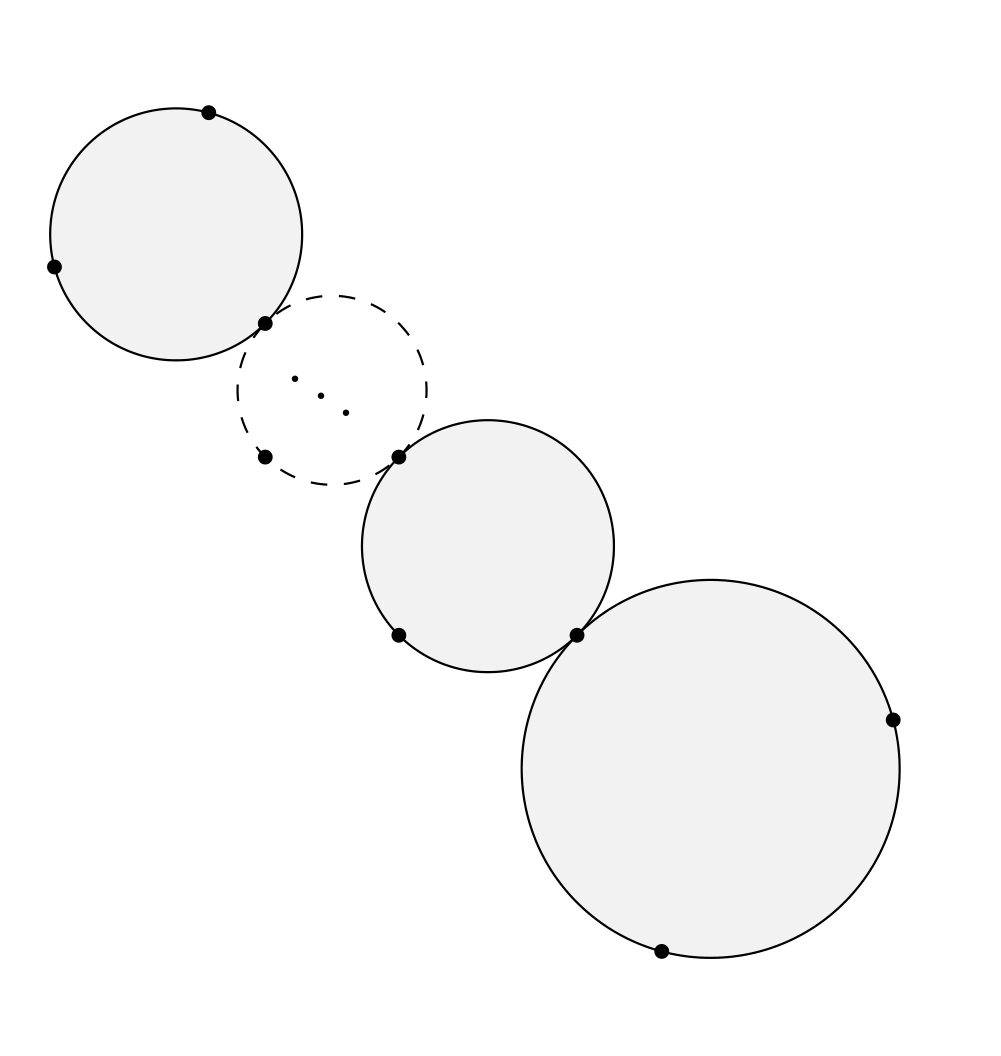
\includegraphics[width=0.44\textwidth]{figures/fig4_4.png}
\caption{三个三标点全纯圆盘构成的单腿树。}
\label{fig:tree}
\end{figure}

$p_1\in U\cap T_1$、$p_k\in U\cap T_k$，以及 $T_i\cong T_{i+1}$ 的恒等元
$a_i\in T_i\cap T_{i+1}$。

\transnote{含糊点拨：底本这一句在 p.72 末只写到「与交点处成角」，p.73 首因插图隔开，
才接上 $p_1\in U\cap T_1,\dots$。译文把「成角：」留在前段、把角点列表接在插图上端，
读起来语义不断。}

现在选取 $\gamma\colon[0,1)\to\overline{\cS}_k$，它是 $(k+1)$ 标点圆盘紧化模空间中
一条光滑简单道路（即一族共形结构），从固定的共形结构 $r=\gamma(0)$ 出发，走向最深的
边界层 $r_0=\lim_{t\to1^-}\gamma(t)$，在那里 $r$ 退化为单腿三叉圆盘树 $r_0$，即单腿树（one-legged tree），
见图 \ref{fig:tree}。现在考虑参数化模空间（parametrized moduli space）
$\widetilde{\cM}_J^{k,\C^2}(p_1,a_1,\dots,a_{k-1},p_k)$：其中的 $(v,s)$ 是 $\C^2$ 中
$J$-全纯圆盘，边界条件与 $u$ 相同，但定义域上的共形结构 $s$ 允许沿道路 $\gamma$ 变动。
标准论证表明，对 $\C^2$ 上一般的近复结构 $J$，该模空间成为光滑的一维流形。再次把前面
关于 $X\times\C$ 上近复结构的构造用于修改后的 $J$（代替 $\C^2$ 上标准近复结构），便知
可以保证：对任何 $(u,r)\in\cM_J^{k,X\times\C}(y_1,x_1,\dots,x_k,y_2)$，$p(u,r)$ 与
$\pi(u,r)$ 也都正则。

\transnote{易错预警：带波浪号的 $\widetilde{\cM}$ 是参数化模空间，其定义域的共形结构
沿道路 $\gamma$ 变动，不要与普通模空间 $\cM$ 混同；$r$ 是共形类，不是半径。}

现在考虑 $\widetilde{\cM}_J^{k,\C^2}(p_1,a_1,\dots,a_{k-1},p_k)$ 的 Gromov 紧化（Gromov compactification）。
对纤维丛 $\C^2\to\C$ 施用极大值原理，该模空间中的圆盘不可能逃逸到无穷远，

% ===== 原书 p.74 =====
因而可施用 Gromov 紧性。正合性排除圆盘泡与球泡（bubbling）；又因 $p_1$、$a_i$、$p_k$ 次数相同，
不会发生条带破裂（strip breaking）。于是
$\widetilde{\cM}_J^{k,\C^2}(p_1,a_1,\dots,a_{k-1},p_k)$ 的边界分支只来自道路 $\gamma$
两端的定义域共形结构。在 $0$ 端，共形结构是 $\gamma(0)=r$，故 Gromov 边界的一部分由
固定共形结构 $r$ 的圆盘模空间给出。在另一端，$\lim_{t\to1^-}\gamma(t)=r_0$；该边界
分支由贡献于迭代乘积运算
\[
\mu^2(\mu^2(\cdots\mu^2(a_1,a_2)\cdots),a_{k-1}),p_k)=p_1
\]
的圆盘组成，其中 $p_k\in U\cap T_k$，$a_i$ 是 $T_i\cong T_{i+1}$ 的恒等元。如上所述，
每个这样的乘积运算在 $\C^2$ 中都有唯一的全纯圆盘表示，因而这样的圆盘只有一个。于是，
由于 $\widetilde{\cM}_J^{k,\C^2}(p_1,a_1,\dots,a_{k-1},p_k)$ 是带边界的一维流形，
在投影 $\pi$ 到 $\C^2$ 下必恰有一个共形类为 $r$ 的圆盘 $(u,r)$。
\end{proof}

现在可以证明主要结果。

\begin{thmstar}
设 $X$ 是光滑仿射簇，带嵌入 $X\to\C^N$，该嵌入在 $X$ 上诱导 Stein 结构；设
$f\colon X\to\C$ 是 $\C^N$ 上多项式函数的限制。若 $f$ 只有一个临界纤维
$f^{-1}(0)$，则对充分小的 $t\neq0$，存在 $A_\infty$ 范畴的拟等价
\[
D^\pi\cW(f^{-1}(t))[s^{-1}]\to D^\pi\cW(X\times\C,zf).
\]
\end{thmstar}

\transnote{易错预警：原书在证明主定理前重述引言中的定理 \ref{thm:knorrer}（导出 Knörrer 周期性），
并沿用编号「1.3.1」。译本同样用无编号的 thmstar 环境，编号引
定理 \ref{thm:knorrer}，以免自动编号另起新号。}

% ===== 原书 p.75 =====
\begin{proof}
这由前面的结果合并得到。把论证明确写出来：
\begin{itemize}
\item 由推论 \ref{cor:2-3-2}，$\cW(f^{-1}(0))$ 是 $\cW(f^{-1}(t))$ 对由形如
$\cap L$ 的拉格朗日子流形生成的子范畴 $\cD'$ 的商；
\item 由命题 \ref{prop:3-0-5}，该子范畴 $\cD'$ 与由 $\cap\ell$（$\ell$ 取遍附加余核）
生成的子范畴相同；
\item 由定理 \ref{thm:aak-equiv}，$\cW(f^{-1}(t))$ 等价于
$\cW(X\times\C,z(f-t))$；在该等价下，$\cD'$ 的生成元 $\cap\ell$ 由
定理 \ref{thm:4-2-1} 送到子范畴 $\cD$ 的对象 $\bigcup\ell$；
\item 由命题 \ref{prop:3-0-4}，$\cW(X\times\C,z(f-t))$ 对子范畴 $\cD$ 的商给出
$\cW(X\times\C,zf)$。
\end{itemize}
于是
\[
D^\pi\cW(f^{-1}(0))\cong D^\pi\cW(f^{-1}(t))/\cD'
\cong D^\pi\cW(X\times\C,z(f-t))/\cD\cong D^\pi\cW(X\times\C,zf).
\]
\end{proof}

\transnote{含糊点拨：$\cD'$ 与 $\cD$ 是两个不同的子范畴：$\cD'$ 由 $f^{-1}(t)$ 一侧的
$\cap L$ 生成，$\cD$ 由 $X\times\C$ 一侧的 $\bigcup\ell$ 生成，定理 \ref{thm:4-2-1}
正是说二者在 AAK 等价下彼此对应。链式同构的三步依次用推论 \ref{cor:2-3-2}、
定理 \ref{thm:aak-equiv} 与命题 \ref{prop:3-0-4}。}
